\documentclass[notes,11pt, aspectratio=169, xcolor=table]{beamer}

\usepackage{pgfpages}
% These slides also contain speaker notes. You can print just the slides,
% just the notes, or both, depending on the setting below. Comment out the want
% you want.
\setbeameroption{hide notes} % Only slide
%\setbeameroption{show only notes} % Only notes
%\setbeameroption{show notes on second screen=right} % Both

\usepackage{helvet}
\usepackage[default]{lato}
\usepackage{array}
\usepackage{minted}

\newtheorem{proposition}{Proposition}

\usepackage{tikz}
\usetikzlibrary{shapes.geometric}
\usepackage{pgfplots}
\usepackage{graphicx}
\usepackage{verbatim}
\setbeamertemplate{note page}{\pagecolor{yellow!5}\insertnote}
\usetikzlibrary{positioning}
\usetikzlibrary{snakes}
\usetikzlibrary{calc}
\usetikzlibrary{arrows}
\usetikzlibrary{decorations.markings}
\usetikzlibrary{shapes.misc}
\usetikzlibrary{matrix,shapes,arrows,fit,tikzmark}
\usepackage{amsmath}
\usepackage{mathpazo}
\usepackage{hyperref}
\usepackage{lipsum}
\usepackage{multimedia}
\usepackage{graphicx}
\usepackage{multirow}
\usepackage{graphicx}
\usepackage{dcolumn}
\usepackage{bbm}
\usepackage[style=authoryear,sorting=nyt,uniquename=false]{biblatex}

\addbibresource{references.bib} 

\newcolumntype{d}[0]{D{.}{.}{5}}

\def\@@mybluebox[#1][#2]#3{
    \sbox\mytempbox{#3}%
    \mytemplen\ht\mytempbox
    \advance\mytemplen #1\relax
    \ht\mytempbox\mytemplen
    \mytemplen\dp\mytempbox
    \advance\mytemplen #2\relax
    \dp\mytempbox\mytemplen
    \colorbox{myblue}{\hspace{1em}\usebox{\mytempbox}\hspace{1em}}}


\usepackage{changepage}
\usepackage{appendixnumberbeamer}
\newcommand{\beginbackup}{
   \newcounter{framenumbervorappendix}
   \setcounter{framenumbervorappendix}{\value{framenumber}}
   \setbeamertemplate{footline}
   {
     \leavevmode%
     \hline
     box{%
       \begin{beamercolorbox}[wd=\paperwidth,ht=2.25ex,dp=1ex,right]{footlinecolor}%
%         \insertframenumber  \hspace*{2ex} 
       \end{beamercolorbox}}%
     \vskip0pt%
   }
 }
\newcommand{\backupend}{
   \addtocounter{framenumbervorappendix}{-\value{framenumber}}
   \addtocounter{framenumber}{\value{framenumbervorappendix}} 
}


\usepackage{graphicx}
\usepackage[space]{grffile}
\usepackage{booktabs}

% These are my colors -- there are many like them, but these ones are mine.
\definecolor{blue}{RGB}{0,114,178}
\definecolor{red}{RGB}{213,94,0}
\definecolor{yellow}{RGB}{240,228,66}
\definecolor{green}{RGB}{0,158,115}
\newcommand{\blue}[1]{\textcolor{blue}{#1}}

\hypersetup{
  colorlinks=false,
  linkbordercolor = {white},
  linkcolor = {blue}
}


%% I use a beige off white for my background
\definecolor{MyBackground}{RGB}{255,253,218}

%% Uncomment this if you want to change the background color to something else
%\setbeamercolor{background canvas}{bg=MyBackground}

%% Change the bg color to adjust your transition slide background color!
\newenvironment{transitionframe}{
  \setbeamercolor{background canvas}{bg=yellow}
  \begin{frame}}{
    \end{frame}
}

\setbeamercolor{frametitle}{fg=blue}
\setbeamercolor{title}{fg=blue}
\setbeamertemplate{footline}[frame number]
\setbeamertemplate{navigation symbols}{} 
\setbeamertemplate{itemize items}{-}
\setbeamercolor{itemize item}{fg=blue}
\setbeamercolor{itemize subitem}{fg=blue}
\setbeamercolor{enumerate item}{fg=blue}
\setbeamercolor{enumerate subitem}{fg=blue}
\setbeamercolor{button}{bg=MyBackground,fg=blue,}



% If you like road maps, rather than having clutter at the top, have a roadmap show up at the end of each section 
% (and after your introduction)
% Uncomment this is if you want the roadmap!
% \AtBeginSection[]
% {
%    \begin{frame}
%        \frametitle{Roadmap of Talk}
%        \tableofcontents[currentsection]
%    \end{frame}
% }
\setbeamercolor{section in toc}{fg=blue}
\setbeamercolor{subsection in toc}{fg=red}
\setbeamersize{text margin left=1em,text margin right=1em} 

\newenvironment{wideitemize}{\itemize\addtolength{\itemsep}{10pt}}{\enditemize}

\usepackage{environ}
\NewEnviron{videoframe}[1]{
  \begin{frame}
    \vspace{-8pt}
    \begin{columns}[onlytextwidth, T] % align columns
      \begin{column}{.58\textwidth}
        \begin{minipage}[t][\textheight][t]
          {\dimexpr\textwidth}
          \vspace{8pt}
          \hspace{4pt} {\Large \sc \textcolor{blue}{#1}}
          \vspace{8pt}
          
          \BODY
        \end{minipage}
      \end{column}%
      \hfill%
      \begin{column}{.42\textwidth}
        \colorbox{green!20}{\begin{minipage}[t][1.2\textheight][t]
            {\dimexpr\textwidth}
            Face goes here
          \end{minipage}}
      \end{column}%
    \end{columns}
  \end{frame}
}

\title[]{International Trade: Lecture 0}
\subtitle[]{Preliminaries}
\author[Góes]
{Carlos Góes\inst{1}}
\date{Fall 2025}
\institute[GWU]{\inst{1} George Washington University }



\begin{document}

%%% TIKZ STUFF
\tikzset{   
        every picture/.style={remember picture,baseline},
        every node/.style={anchor=base,align=center,outer sep=1.5pt},
        every path/.style={thick},
        }
\newcommand\marktopleft[1]{%
    \tikz[overlay,remember picture] 
        \node (marker-#1-a) at (-.3em,.3em) {};%
}
\newcommand\markbottomright[2]{%
    \tikz[overlay,remember picture] 
        \node (marker-#1-b) at (0em,0em) {};%
}
\tikzstyle{every picture}+=[remember picture] 
\tikzstyle{mybox} =[draw=black, very thick, rectangle, inner sep=10pt, inner ysep=20pt]
\tikzstyle{fancytitle} =[draw=black,fill=red, text=white]
%%%% END TIKZ STUFF



%----------------------------------------------------------------------%
%-------------------       TITLE PAGE       ---------------------------%
%----------------------------------------------------------------------%





%----------------------------------------------------------------------%






%----------------------------------------------------------------------%
%----------------------------------------------------------------------%

%----------------------------------------------------------------------%
\frame{\titlepage}
\addtocounter{framenumber}{-1}
%----------------------------------------------------------------------%



%----------------------------------------------------------------------%
%----------------------------------------------------------------------%

\section{Housekeeping}

\begin{frame}{Outline}
\begin{wideitemize}
\item About me
\item Course objectives and organization
\item Some initial topics for debate
    
\end{wideitemize}

\end{frame}


\begin{frame}{About me}

\begin{columns}[T] % align columns
\begin{column}{.38\textwidth}
I'm originally from Brazil...
\vspace{10cm}
  \makebox[\linewidth][c]{
    \resizebox{\linewidth}{!}{
    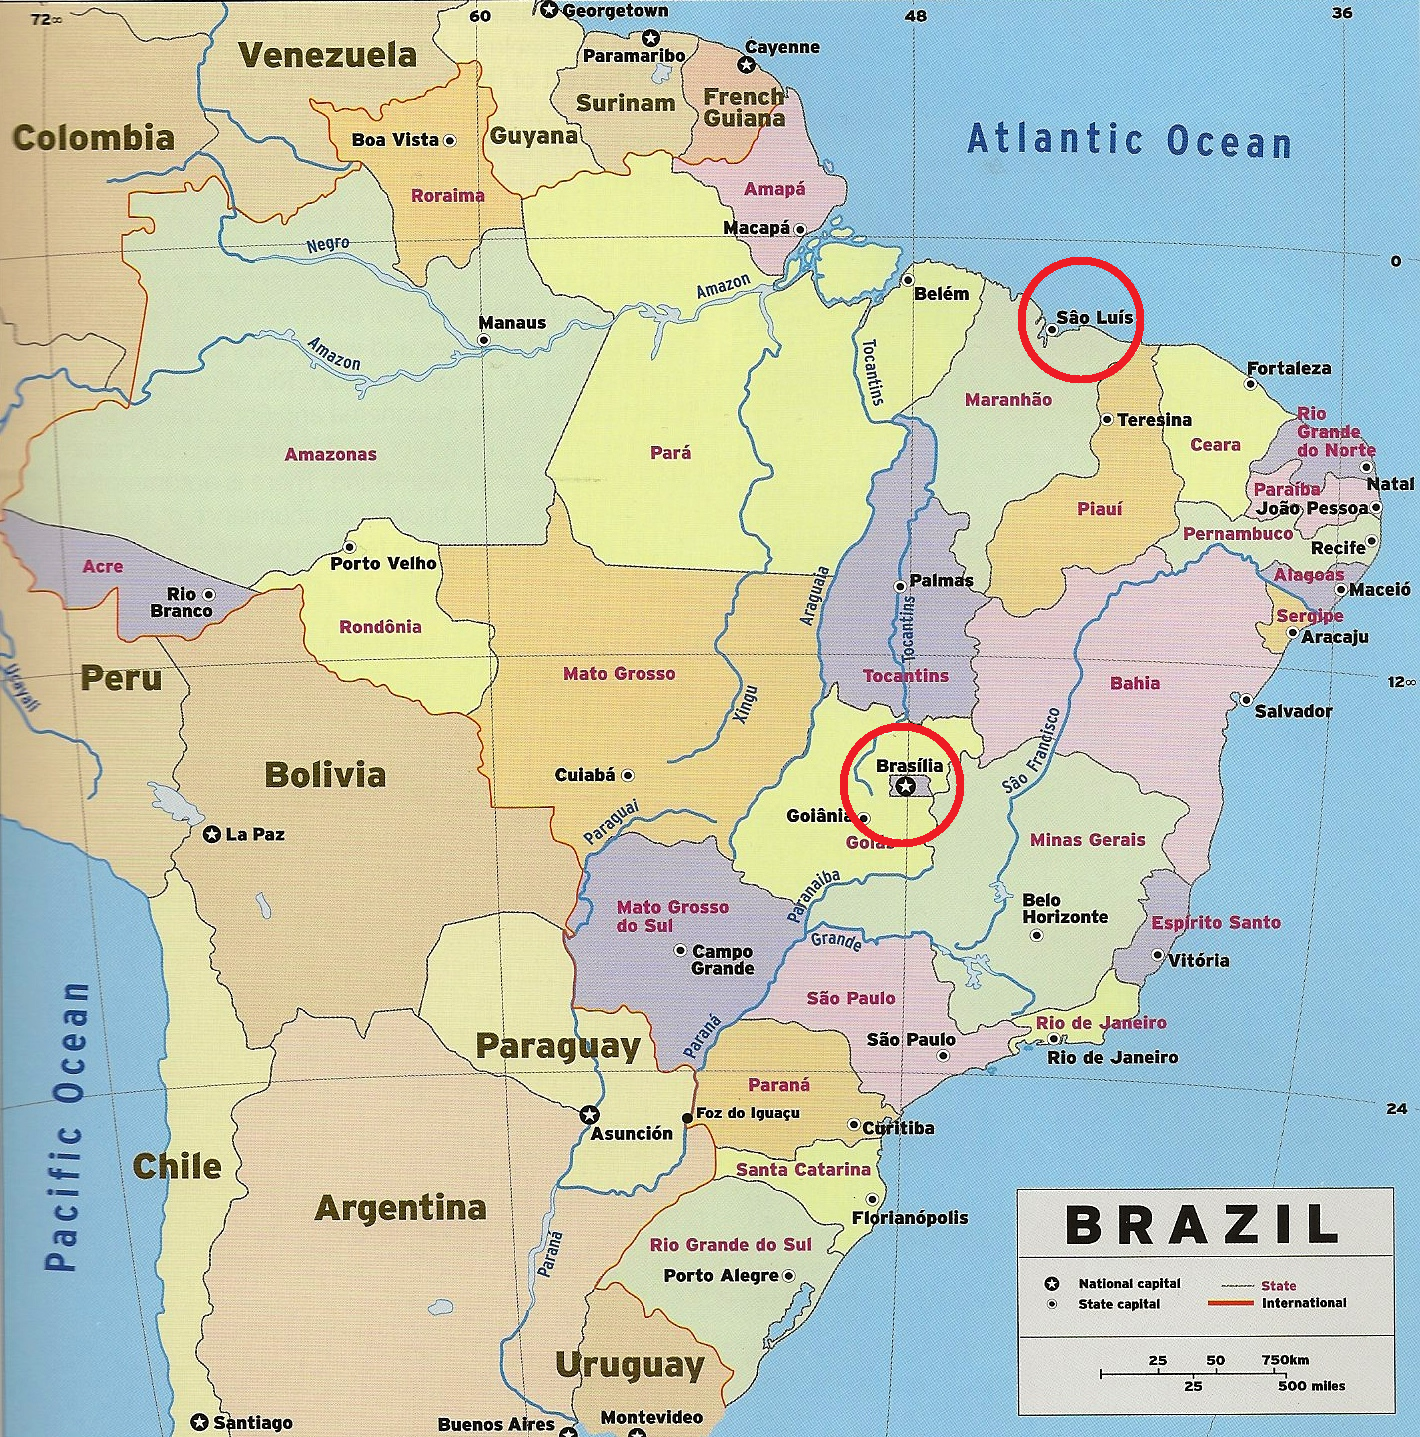
\includegraphics{figs/brazil.png}
      }
    }
\end{column}%
\hfill%
\begin{column}{.58\textwidth}
  \begin{wideitemize}
    \item Education:
    \begin{itemize}
        \item Ph.D.: University of California, San Diego 
        \item M.A.: Johns Hopkins SAIS 
        \item B.A.: University of Brasilia 
    \end{itemize}
    \item Professional:
    \begin{itemize}
        \item Economist, World Bank Group 
        \item Research Economist, World Trade Organization
        \item Senior Economic Advisor, President of Brazil
    \end{itemize}    
    \item Misc:
    \begin{itemize}
        \item Twitter: @goescarlos
        \item Website: www.carlosgoes.com
    \end{itemize}    
    \item Research: Macro \& International Trade
  \end{wideitemize}
\end{column}%
\end{columns}
\end{frame}


\begin{frame}{Course objectives}
\begin{wideitemize}
\item International Trade Theory and Policy (ECON 2181).
\item Course objectives:
    \begin{enumerate}
        \item \blue{Comprehend and explain} the modern trade theories and their assumptions;
        \item \blue{Illustrate} each theory using standard analytical tools (e.g., PPFs, GE diagrams, gravity) and data;
        \item \blue{Solve} for the equilibrium of different models, using pen-and-paper as well as a computer;
        \item \blue{Interpret policy implications} and distributional effects of trade and trade policy.
    \end{enumerate}

\end{wideitemize}    
\end{frame}

\begin{frame}{What do you need to know in the beginning of this course?}

\begin{wideitemize}
        \item Pre-reqs: ECON 1011 and ECON 1012
        \item Most of you are econ majors, so I expect you to have heard of:
        \begin{enumerate}
            \item Indifference curves
            \item Production functions / production possibility sets
            \item Equilibrium
        \end{enumerate}
        \item<2-> I expect you know how to take a derivative (or be willing to re-learn how to do it)
        \item<3-> Most cases, I will make your life easier and write down a simple maximization problem
        \item<4-> This is \textbf{not} a mathematical economics course: no long, detailed, rigorous proofs

        \item<5-> However, math is important. And basic calculus + algebra helps with the intuition. You should be able to do it.

\end{wideitemize}
    
\end{frame}


\begin{frame}{Textbook}

\begin{columns}[T] % align columns
\begin{column}{.4\textwidth}
  \makebox[\linewidth][c]{
    \resizebox{\linewidth}{!}{
    \includegraphics{figs/KOM-IT.png}
      }
    }
\end{column}%
\hfill%
\begin{column}{.58\textwidth}
  \begin{wideitemize}
  \item \textit{International Trade: Theory and Policy.}
    \item Edition: 11th
    \item Authors:
  \begin{itemize}
    \item Paul Krugman (Nobel)
    \item Maurice Obstfeld (former IMF Chief)
    \item Marc Melitz (future Nobel)
  \end{itemize}
  \end{wideitemize}
\end{column}%
\end{columns}
\end{frame}

\begin{frame}{Handouts}

\begin{columns}[T] % align columns
\begin{column}{.4\textwidth}
  \makebox[\linewidth][c]{
    \resizebox{\linewidth}{!}{
    \includegraphics{figs/handout.jpg}
      }
    }
\end{column}%
\hfill%
\begin{column}{.58\textwidth}
  \begin{wideitemize}
  { \scriptsize
  \item I have prepared handouts that will cover all of the theoretical models and expand on the textbook
  \item<2-> They are more complete, in the sense that I write down the math and explain step by step how to get there
  \item<3-> The textbook sometimes require you to ``just trust me, bro''... and I always found that a bit unsatisfactory (even as an undergrad).
  \item<4-> They are \textit{too complete} in the sense that they cover \textit{more} than what is required to do well in this course
  \item<5-> But they are a great resource, especially if you are in doubt or  want to go deeper
  \item<6-> I also prepared them from scratch! You are the first to use them. If you find typos, let me know.
  }
  \end{wideitemize}
\end{column}%
\end{columns}
\end{frame}

\begin{frame}{Grading}
\begin{wideitemize}
    \item Course grades are based on two midterms, one final, code assignments, and two mini-projects:

\medskip
\begin{tabular}{l r}
Code assignments & 15\% \\
Mini-Project 1 & 5\% \\
Mini-Project 2 & 5\% \\
Midterm & 30\% \\
Final Exam (cumulative) & 45\%
\end{tabular}

\medskip
\noindent Details, rubrics, and deadlines will be posted online. Limited extra credit may be awarded for \textit{constructive, regular class participation}.


\end{wideitemize}    
\end{frame}


\begin{frame}{Policies (i)}
\begin{wideitemize}
    \item \textcolor{blue}{Attendance}
    \begin{itemize}
        \item I do not require attendance
        \item You are an adult and I will treat you as such
        \item If you skip all the classes and do well in my class, congrats (low probability)
        \item If you attend all classes and follow the slides, you will get a good grade (high probability) 
    \end{itemize}

\onslide<2->{
     \item \textcolor{blue}{Honesty and regrading policy}
    \begin{itemize}
        \item The main rule is: do not be dishonest (you will get caught)
        \item If you have a problem, let me know in advance -- I am reasonable
        \item Regrade policy: arithmetical error (I summed scores wrong); or full exam regrade (your score might go up or down)
        \item You cannot appeal on a single question
        \end{itemize}   
}
\end{wideitemize}    
\end{frame}

\begin{frame}{Policies (ii)}

\begin{wideitemize}
    \item \blue{Exams}
    \begin{itemize}
        \item No make-up exams are offered.
        \item You can choose to skip the midterm and increase the weight of your final exam.
        \item Late homework is not accepted without a qualifying emergency.
        \item Religious exceptions also follow GW policy.
        \item Final exam scheduling follows the official GW schedule.
    \end{itemize}
    \item<2-> \blue{Collaboration}
    \begin{itemize}
        \item You are encouraged to discuss problem sets conceptually with peers
        \item The work you submit must be your own.
        \item All submitted work must reflect your independent understanding.
        \item tl;dr work together. don't copy. it's a waste of your family's (or the govt's, or your future self's) money.
    \end{itemize}

\smallskip



\end{wideitemize}
    
\end{frame}

\begin{frame}{Policies (iii)}

\begin{wideitemize}
    \item  \textcolor{blue}{Technology}
    \begin{itemize}
        \item For take-home exercises, you can use whatever tools you want, including AI
        \item<2-> Unless I explicitly prohibit the use of generative AI, you can use it for this course
        \item<3-> AI can be quite useful as a tutor or helper in studying. I use it daily, particularly for coding or deep research.
        \item<4-> But... note the following:
        \begin{enumerate}
            \item you are responsible for everything you submit;
            \item ``ChatGPT'' is not a source -- you need to go to original sources and verify the claims;
            \item you should ground your claims on reputable sources (peer reviewed research; reports from the IMF, World Bank, WTO, OECD, etc)
            \item you need to type/write the answers yourself -- in other words, you can't copy and paste images or texts out of ChatGPT into the answers
        \end{enumerate}
        
        \item<5-> AI can be your friend (I encourage it) but it's an assistant not a replacement for effort
    \end{itemize}

\end{wideitemize}
    
\end{frame}

\begin{frame}[fragile=singleslide]{When you have domain knowledge, AI can be your friend}

\begin{minted}[breaklines, fontsize=\tiny]{markdown}
    # Context 
    
    Research project that tries to understand economic networks in the context of multiple sectors and heterogeneous firms. Firms of different sizes have different constraints and optimal policy might want to focus on firms that are close to their constraints to fix market failures. Empirically, you are trying to understand how small and medium enterprises fall within supply chains and economic networks, particularly in developing countries.
    
    # Goal
    
    Do a comprehensive literature review of:
    
    - The economic networks literature, from a theory/modelling. Be clear on how this relates and/or differs from supply chains or global value chains (or if they are all different words for the same object). You can focus on papers that use both a partial equilibrium or general equilibrium approach;
    - The empirical literature on supply chains/economic networks, focusing particularly on developing countries. Research summarize papers that take descriptive approaches to economic networks. Also research and summarize empirical papers that have a causal claim, describing both the empirical models they use and how credible is the identification strategy they might have used.
    - The heterogeneous firms literature, particularly where it focuses on developing countries. This includes the main papers on heterogeneous firms (a la Aiyagari or HANK) and misallocation (a la Klenow and Hsieh). Research extensions of these canonical models to (a) multiple sectors; (b) relationships with supply chains/economic networks; and (c) developing countries.
    - Relevant reports by multilateral organizations such as the World Bank, the IMF, the WTO and others on the topic of economic networks.
\end{minted}


    
\end{frame}


\begin{frame}{Code assingments}

\begin{wideitemize}
    \item We will have a series of Data Labs throughout the semester
    \item<2-> The idea is to introduce you to Python and its uses for data science and economics 
    \item<3-> Five data labs in total
    \item<4-> After three of them (TBD), you will be required to submit a coding assignment. 
    \item<5-> Each will be worth $5\%$ of your grade.

\textit{Tentative deadlines:} one week after each data lab that requires an assignment.

\end{wideitemize}
 


    
\end{frame}

\begin{frame}{Data + coding}
\begin{wideitemize}
    \item \textcolor{blue}{Coding}
    \begin{itemize}
        \item Aside from trade knowledge, I want you to get skills out of this class
        \item I will ask you to download data, transform it using computer code, plot charts and tables
        \item If you don't know how, don't freak out... I'll help you (also, use Google + AI). Learn!
    \end{itemize}
\onslide<2->{
    \item \textcolor{blue}{Python}
    \begin{itemize}
        \item Python is a general purpose language... people actually code apps with it
        \item It is also very useful for data science:
        \begin{itemize}
            \item downloading data
            \item transforming data
            \item using statistics to summarize or correlate it
            \item plotting charts and maps
        \end{itemize}
    \end{itemize}
}
\onslide<3->{
    \item \textcolor{blue}{Anaconda}
    \begin{itemize}
        \item Free + open source distribution
        \item Optimized for data science
        \item \url{https://www.anaconda.com/download}
        \item Installing + exploring lab soon
    \end{itemize}
}
\end{wideitemize}    
\end{frame}

\begin{frame}{Problem sets}
\begin{wideitemize}
    \item I will assign a subset of the textbooks exercises as practice problem sets.
    \item They will not be graded but will serve as practice for your midterm and final.
    \item I will use some exercises that show up in your problem sets in the exams.
    \item You do have to do them... but if you do, chances are you will do better in the exams.

\end{wideitemize}
    
\end{frame}

\begin{frame}{Key dates}
\begin{wideitemize}
    \item Midterm: Thu, Oct 16
    \item Final: Per official GW exam schedule (time/place TBA on Blackboard, on Finals week)
    \item I might need to travel for work some days... if that happens, we will host some asynchronous remote classes + office hours by appointment.
\end{wideitemize}    
\end{frame}

\begin{frame}{Why do we trade?}
\begin{wideitemize}
    \item Have you engaged in trade today?
\onslide<3->{
    \begin{itemize}
        \item You all are trading your future (hopefully higher) income for my teaching;
        \item I am teaching so that I can pay for my wife's handbags;
    \end{itemize}
}
\onslide<3->{
    \item What makes countries (or people) trade?
}
\onslide<4->{
    \vspace{12pt}

    \begin{itemize}
        \item Different skills (e.g., I am bad mechanic, so I pay Jiffy Lube instead)
        \item Different endowments (e.g., Saudi Arabia has a lot of oil; Luxembourg does not);
        \item Different products (e.g., both France and Italy produce wine, but trade for variety);
    \end{itemize}
}
\end{wideitemize}    
\end{frame}

\begin{frame}{Some misconceptions about comparative advantage}
\begin{wideitemize}
    \item ``Free trade is only beneficial if a country is productive enough to compete.'' \\
    \qquad No. Trade is beneficial if there is a comparative advantage. Absolute disadvantage does not matter.

    \item<2-> ``Free trade lowers income in low-wage countries.'' \\
    \qquad No. Trade is beneficial if there is a comparative advantage. Absolute wages do not matter.

    \item<3-> ``Free trade makes us poorer because we spend money on other countries goods.'' \\
    \qquad No. Having access to more affordable goods makes us better off by specializing and trading.

    \item<4-> ``Free trade closes the income gap between poor and rich countries.'' \\
    \qquad No. Trade raises every country’s welfare beyond autarky welfare. Per capita
income differences remain, and depend on a country’s production possibilities.

\end{wideitemize}
    
\end{frame}



\begin{frame}{How to survive political memes}

\begin{figure}
    \centering
    \includegraphics[width=0.5\linewidth]{figs/meme2.jpg}
\end{figure}

    
\end{frame}


\begin{frame}{Some answers}

\begin{wideitemize}
    \item While free trade makes society (in general) better off not everyone gains from it
    \begin{itemize}
    \item Over the LR, all resources are mobile, economy readjusts optimally
    \item Over the SR, some factors may be immobile
   
        \item Land is scarce, if the price of agricultural goods falls with imports, landowners lose
        \item Losses are concentrated in a few sectors; gains are dispersed in society
        \item Politically, losers are more organized
    \end{itemize}
    
    \item<2-> It's hard to collect taxes
    \begin{itemize}
        \item You need a complicated bureaucracy like the IRS to enforce tax law
        \item You need firms and households to apply complicated formulas
        \item You need electronic bookkeeping to ensure sales taxes are not evaded within a country
        \item Lack of state capacity means some countries (particularly poor countries) use tariffs instead
        \item You only need to enforce them once goods cross borders
    \end{itemize}
    

\end{wideitemize}

    
\end{frame}


\begin{frame}{Some answers (ii)}

\begin{wideitemize}
    \item Some industries have ``scale economies''
    \item This means the average cost of producing something decreases in the size of production
    \item<2-> Some countries try to protect ``infant industries'' with hopes they achieve competitiveness 
    \item<3-> In some cases, that has worked (Chemical industries in Korea)
    \item<4-> More often than not, it has not
    \item<5-> If it doesn't the outcome is:
    \begin{itemize}
        \item harming the consumer, by preventing them from accessing cheaper and/or higher quality foreign goods
        \item keeping unproductive firms in the market (misallocation)
    \end{itemize}
    
\end{wideitemize}

    
\end{frame}



\begin{frame}{Other topics}

\begin{wideitemize}
    \item Can we still trade even if a country is more productive in everything?
    \item Who gains and who loses with trade?
    \item What happens with exports after countries grow in endowment?
    \item Why do we trade within the same industry (e.g., cars for cars)?
    \item What happens with firms after trade?
\end{wideitemize}

    
\end{frame}

\end{document}
